\documentclass[aspectratio=169,handout]{beamer}
% \usepackage[utf8]{inputenc}
\usetheme{metropolis}
\usecolortheme{orchid}
\usepackage{amsmath}
\usepackage{amssymb}
\usepackage{amsthm}
\usepackage{multirow}
\usepackage[ruled]{algorithm2e}
\usepackage{mathtools}
\usepackage{caption}
% \usepackage{epstopdf}
\usepackage{hyperref}
\usepackage{subcaption}
\usepackage{siunitx}
\usepackage{textcomp}
\usepackage{tcolorbox}
\usepackage{tikz}
\usetikzlibrary{tikzmark,positioning,arrows.meta,shapes.misc,calc}

\setbeamerfont{footnote}{size=\tiny}

% Information boxes
\newcommand*{\info}[4][16.3]{%
  \node [ annotation, #3, scale=0.65, text width = #1em,
          inner sep = 2mm ] at (#2) {%
  \list{$\bullet$}{\topsep=0pt\itemsep=0pt\parsep=0pt
    \parskip=0pt\labelwidth=8pt\leftmargin=8pt
    \itemindent=0pt\labelsep=2pt}%
    #4
  \endlist
  };
}

%% Definitions for root locus plots
\newcommand*{\rootlocusexample}[4]{% xmin,xmax,ymin,ymax,
		\foreach \x in {#1,...,#2}{
			\ifthenelse{\x=0}{}
		  {% false case
   			\draw (\x cm,1pt) -- (\x cm,-1pt) node[anchor=north] {$\x$};
		  }
		}
		\foreach \y in {#3,...,#4}{
			\ifthenelse{\y=0}{}
		  {% false case
   			\draw (-1pt,\y cm) -- (1pt,\y cm) node[anchor=east] {$\y$};
		  }
   	}
		\draw [-latex] (#1,0) -- (#2,0) node [above]  {$\sigma$};
		\draw [-latex] (0,#3) -- (0,#4) node [right] {$j\omega$};
}

\def\centerarc[#1](#2)(#3:#4:#5)% Syntax: [draw options] (center) (initial angle:final angle:radius)
    { \draw[#1] ($(#2)+({#5*cos(#3)},{#5*sin(#3)})$) arc (#3:#4:#5); }

\tikzset{%
  >={Latex[width=2mm,length=2mm]},
  % Specifications for style of nodes:
            base/.style = {rectangle, rounded corners, draw=black,
                           minimum width=4cm, minimum height=1cm,
                           text centered, font=\sffamily},
  activityStarts/.style = {base, fill=blue!30},
       startstop/.style = {base, fill=red!30},
    activityRuns/.style = {base, fill=green!30},
         process/.style = {base, minimum width=2.5cm, fill=orange!15,
                           font=\ttfamily},
}

\tikzset{pole/.style={cross out, draw=black, minimum size=2*(#1-\pgflinewidth), inner sep=0pt, outer sep=0pt},
pole/.default={3pt}}
\tikzset{poledes/.style={rectangle, draw=black, minimum size=2*(#1-\pgflinewidth), inner sep=0pt, outer sep=0pt},
poledes/.default={3pt}}
\tikzset{zero/.style={circle, draw=black, fill=white, minimum size=2*(#1-\pgflinewidth), inner sep=0pt, outer sep=0pt},
zero/.default={3pt}}
\tikzset{test/.style={rectangle, draw=black, fill=white, minimum size=2*(#1-\pgflinewidth), inner sep=0pt, outer sep=0pt},
test/.default={3pt}}

%% Definitions for block diagrams
\tikzstyle{block} = [draw, fill=blue!20, rectangle, 
    minimum height=2em, minimum width=3em]
\tikzstyle{sum} = [draw, fill=blue!20, circle, node distance=1cm]
\tikzstyle{input} = [coordinate]
\tikzstyle{output} = [coordinate]
\tikzstyle{pinstyle} = [pin edge={to-,thin,black}]

\renewcommand\textbullet{\ensuremath{\bullet}}
\newcommand\scalemath[2]{\scalebox{#1}{\mbox{\ensuremath{\displaystyle #2}}}}
\newcommand{\norm}[1]{\left\lVert#1\right\rVert}

%%% Bibliography
\usepackage[citestyle=numeric,style=numeric,backend=biber,doi=false,isbn=false,url=false]{biblatex}
\addbibresource{references.bib}

%%% Suppress biblatex annoying warning
\usepackage{silence}
\WarningFilter{biblatex}{Patching footnotes failed}

%%% new theorems %%%%%%%%%%%%%%%%%%%%%%%%%%%%%%%%%%%%%%%%%%%%%%%%%%%%%%%%%%%%%%
\theoremstyle{definition}
\newtheorem{mydef}{Definition}

\theoremstyle{plain}
\newtheorem{mylemma}{Lemma}[section]
\newtheorem{mytheorem}{Theorem}[section]
\newtheorem{myproposition}{Proposition}[section]
\newtheorem{myproblem}{Problem}[section]
\newtheorem{mydefinition}{Definition}[section]
\newtheorem{myassumption}{Assumption}[section]

\theoremstyle{remark}
\newtheorem{myremark}{Remark}[section]

\newcounter{saveenumi}
\newcommand{\seti}{\setcounter{saveenumi}{\value{enumi}}}
\newcommand{\conti}{\setcounter{enumi}{\value{saveenumi}}}

\resetcounteronoverlays{saveenumi}

\title{Controles}
\subtitle{\small Clase 7: Diseño de Compensadores por LGR - Adelanto, Atraso, Adelanto-Atraso}
\author{Gerardo Becerra, Ph.D.}
\institute{Pontificia Universidad Javeriana\\ Departamento de Electrónica}
\date{Marzo 11, 2020}

\begin{document}

\frame{\titlepage}	

\begin{frame}[<+->]\frametitle{Introducción}
\vspace*{5mm}
\centering
\begin{itemize}
	\item Lugar de las raíces $\rightarrow$ puede indicar que no se pueden lograr el desempeño deseado simplemente modificando una ganancia.
	\item En éstos casos es necesario cambiar la forma del lugar de las raíces para lograr las especificaciones deseadas.
	\item El problema de control involucra insertar un compensador en el sistema.
	\item Compensación $\rightarrow$ diseño de un filtro cuyas carasterísticas tienden a compensar las características no deseadas de la planta.
	\item Diseño usando LGR: cambiar la forma del lugar de las raíces agregando polos y ceros para forzar a las raíces a pasar por las ubicaciones de los polos deseados.
\end{itemize}
\end{frame}

\section{Compensación en Adelanto}
\begin{frame}[<+->]\frametitle{Compensación en Adelanto}
\begin{columns}
	\begin{column}{0.5\textwidth}
	\begin{figure}
		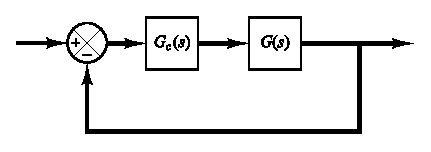
\includegraphics[width=5cm]{images/controlSystem.eps}
	\end{figure}
	\vspace*{-3mm}
	\begin{itemize}
		\item Compensador en serie con la planta $G(s)$.
		\item El problema principal involucra decidir la ubicación de los polos y ceros del compensador $G_c(s)$ para tener polos dominantes de lazo cerrado en las ubicaciones deseadas tal que se cumplan los requerimientos de desempeño.
	\end{itemize}
	\end{column}
	\begin{column}{0.5\textwidth}
	\begin{itemize}
		\item LGR es útil cuando se tienen las especificaciones en términos de la respuesta de tiempo ($\zeta$, $\omega_n$, $T_s$, $PO$, etc).
		\item Considere una planta inestable para cualquier $G_c(s) = K$, o estable pero con un desempeño indeseable durante la respuesta transitoria.
		\item El problema puede resolverse insertando un compensador en adelanto en cascada con la planta.
	\end{itemize}
	\end{column}
\end{columns}
\end{frame}

\begin{frame}[<+->]\frametitle{Procedimiento de Diseño para el Compensador en Adelanto usando LGR}
	\begin{enumerate}
		\item Usando las especificaciones de desempeño, determinar la ubicación deseada de los polos dominantes de lazo cerrado.
		\item Obtener el LGR del sistema no compensado y determinar si ajustando la ganancia $K$ se pueden ubicar los polos en el lugar deseado. Si no, calcular la deficiencia de ángulo $\phi$. Éste ángulo debe ser proporcionado por el compensador en adelanto.
		\item Asumir la forma del compensador en adelanto como
		\begin{equation*}
			G_c(s) = K_c \frac{s+\frac{1}{T}}{s+\frac{1}{\alpha T}}, \hspace*{3mm} 0 < \alpha < 1
		\end{equation*}
		donde $\alpha$ y $T$ se determinan a partir de la deficiencia de ángulo, y $K_c$ se determina del requerimiento de ganancia de lazo abierto.
		\seti
	\end{enumerate}
\end{frame}

\begin{frame}[<+->]\frametitle{Procedimiento de Diseño para el Compensador en Adelanto usando LGR}
	\begin{enumerate}
		\conti
		\item Si no se especifican constantes de error estático dentro de los requerimientos de desempeño, determinar la ubicación del polo y cero del compensador tal que el compensador contribuya el ángulo necesario $\phi$. Buscar hacer $\alpha$ lo más grande posible.
		\item Determinar el valor de $K_c$ del compensador a partir de la condición de magnitud.
		\item Verificar si el compensador diseñado satisface los requerimentos de desempeño. En caso contrario, repetir el proceso de diseño ajustando la ubicación del polo y cero del compensador.
	\end{enumerate}
\end{frame}

\begin{frame}[c]\frametitle{Procedimiento de Diseño Compensador en Adelanto usando LGR - Ejemplo}
\vspace*{2mm}
\begin{columns}
	\begin{column}{0.3\textwidth}
	\begin{figure}
		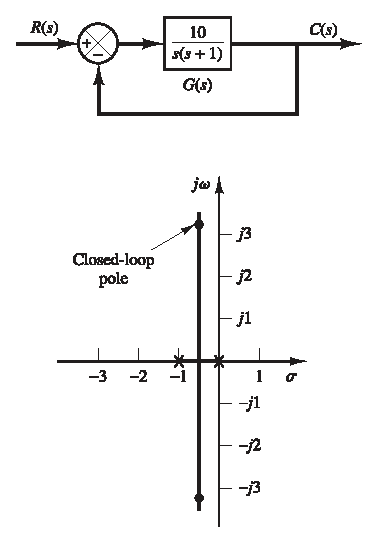
\includegraphics[width=4cm]{images/ejemplo1_planta.eps}
	\end{figure}
	\end{column}
	\begin{column}{0.7\textwidth}
		Considere el sistema de control presentado en la figura. La función de transferencia de la planta es:
		\begin{equation*}
			G(s) = \frac{10}{s(s+1)}		
		\end{equation*}
		\pause
		La función de transferencia de lazo cerrado es:
		\begin{equation*}
			\frac{C(s)}{R(s)} = \frac{10}{s^2+s+10}
		\end{equation*}
		\pause
		Los polos de lazo cerrado están ubicados en $s = -0.5 \pm j3.1225$.
		El factor de amortiguamiento es $\zeta = 0.5/\sqrt{10} = 0.1581$.
		La frecuencia natural es $\omega_n = \sqrt{10} = 3.1623$ rad/s.
		Amortiguamiento pequeño $\Rightarrow$ sobrepico grande (no es deseable!)
	\end{column}
\end{columns}
\end{frame}

\begin{frame}[c]\frametitle{Procedimiento de Diseño Compensador en Adelanto usando LGR - Ejemplo}
	\vspace*{5mm}
	\begin{columns}
		\begin{column}{0.4\textwidth}
			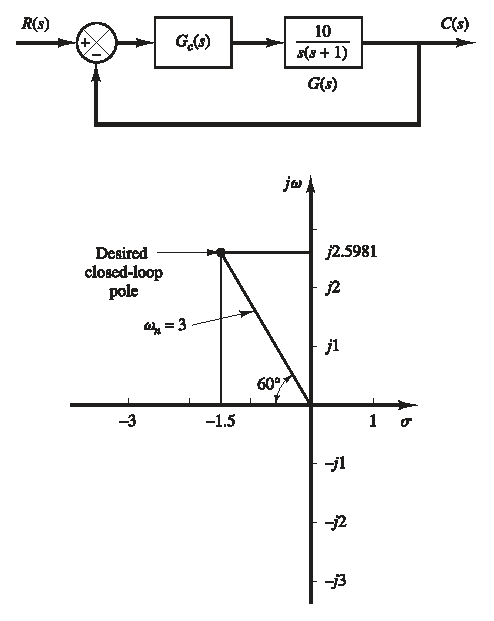
\includegraphics[width=5cm]{images/ejemplo1_compensador.eps}	
		\end{column}
		\begin{column}{0.6\textwidth}
			Se desea un compensador $G_c(s)$ tal que los polos de lazo cerrado tengan $\zeta = 0.5$ y $\omega_n =3$ rad/s. Entonces los polos deseados son:
			\begin{align*}
				s^2 + 2\zeta \omega_n s + \omega_n^2 = s^2 + 3s + 9 = 0\\
				s = -1.5 \pm j2.5981
		 	\end{align*}
		 	\pause
		 	Los polos deseados no se encuentran dentro del LGR del sistema sin compensar $\Rightarrow$ no es suficiente con cambiar la ganancia $K$ $\Rightarrow$ Se requiere introducir un compensador.
		\end{column}
	\end{columns}
\end{frame}

\begin{frame}[c]\frametitle{Procedimiento de Diseño Compensador en Adelanto usando LGR - Ejemplo}
Usando la condición de ángulo se puede verificar que en este caso los polos deseados no se encuentran en el LGR:
\pause
\begin{align*}
	&\sum_{i=1}^M \angle(s+z_i) - \sum_{j=1}^n \angle(s+p_j)\\
	&= -\angle(s) - \angle(s+1)\\
	&= -\ang{120} - \ang{100.894}\\
	&= -\ang{220.894} = \ang{139.106} \neq \ang{180}
\end{align*}
\pause
Entonces, el compensador en adelanto debe contribuir un ángulo $\phi$:
\begin{equation*}
	\phi = \ang{180} - \ang{139.106} = \ang{40.894}
\end{equation*}
\pause
La selección del polo y cero del compensador no es única. A continuación se muestra una forma para hacerlo.
\end{frame}

\begin{frame}[<+->]\frametitle{Procedimiento de Diseño Compensador en Adelanto usando LGR - Ejemplo}
\vspace*{3mm}
\begin{columns}
	\begin{column}{0.3\textwidth}
	\begin{figure}
		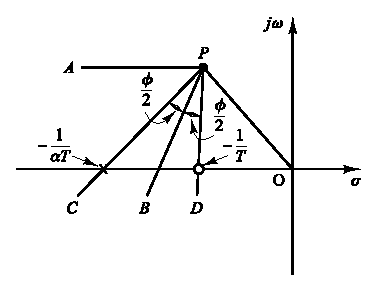
\includegraphics[width=4cm]{images/ejemplo1_poloycero.eps}
	\end{figure}
	\end{column}
	\begin{column}{0.7\textwidth}
		Ubicación de polo y cero:
		\begin{enumerate}
			\item Dibujar una linea horizontal $PA$ que pase a través de $P$, correspondiente a uno de los polos dominantes deseados.
			\item Dibujar la línea $PO$ que conecta a $P$ con el origen.
			\item Dibujar la bisectriz $PB$ del ángulo formado por $PA$ y $PO$.
			\item Dibujar las líneas $PC$ y $PD$ que forman ángulos $\phi/2$ con la bisectriz $PB$.
			\item Ubicar el polo y cero del compensador en adelanto en las intersecciones con el eje real negativo de $PC$ y $PD$, respectivamente.
		\end{enumerate}
	\end{column}
\end{columns}
\end{frame}

\begin{frame}[<+->]\frametitle{Procedimiento de Diseño Compensador en Adelanto usando LGR - Ejemplo}
\begin{columns}
	\begin{column}{0.5\textwidth}
	\begin{figure}
		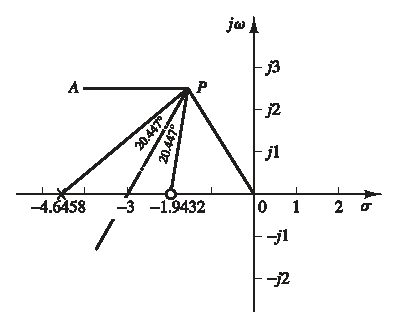
\includegraphics[width=7cm]{images/ejemplo1_poloycero2.eps}
	% \begin{tikzpicture}
	% 	\rootlocusexample{-5}{1}{-1}{3}
	% 	\node[pole,draw=black] at (0,0) {};
	% 	\node[pole,draw=black] at (-1,0) {};
	% 	\node[poledes,draw=black] at (-1.5,2.5981) {};
	% 	\node[zero,draw=black] at (-1.9432,0) {};
	% 	\node[pole,draw=black] at (-4.6458,0) {};
	% 	\draw [dashed] (0,0) -- (-1.5,2.5981) {};
	% 	\draw [dashed] (-1.5,2.5981) -- (-4,2.5981) {};
	% 	\draw [dashed] (-1.5,2.5981) -- (-3,0) {};
	% 	\draw [dashed] (-1.5,2.5981) -- (-1.9432,0) {};
	% 	\draw [dashed] (-1.5,2.5981) -- (-4.6458,0) {};
	% 	\node at (-1.9,1.5) {\small $\frac{\phi}{2}$};
	% 	\node at (-2.3,1.7) {\small $\frac{\phi}{2}$};
	% \end{tikzpicture}
	\end{figure}
	\end{column}
	\begin{column}{0.5\textwidth}
		\begin{itemize}
			\item Ángulo $PA$, $PO$ = \ang{120}
			\item Bisectriz = \ang{60} respecto a $PO$.
			\item Cero en $s = -1.9432$.
			\item Polo en $s = -4.6458$
			\item Entonces, el compensador está dado por:
			\begin{equation*}
				G_c(s) = K_c \frac{s+\frac{1}{T}}{s+\frac{1}{\alpha T}} = K_c\frac{s+1.9432}{s+4.6458}
			\end{equation*}
			con $\alpha = 1.9432/4.6458 = 0.418$.
		\end{itemize}	
	\end{column}
\end{columns}
\end{frame}

\begin{frame}[c]\frametitle{Procedimiento de Diseño Compensador en Adelanto usando LGR - Ejemplo}
	\vspace*{2mm}
	\begin{columns}
		\begin{column}{0.5\textwidth}
			El valor de $K_c$ puede determinarse usando la condición de magnitud:
			\begin{equation*}
				\left| K_c \frac{s+1.9432}{s+4.6458} \frac{10}{s(s+1)}\right|_{s = -1.5+j2.5981} = 1
			\end{equation*}
			\pause
			\begin{equation*}
				K_c = \left| \frac{(s+4.6458)s(s+1)}{10(s+1.9432)} \right|_{s = -1.5+j2.5981} = 1.2287
			\end{equation*}
			\pause
			El compensador diseñado es:
			\begin{equation*}
				G_c(s) = 1.2287 \frac{s+1.9432}{s+4.6458}
			\end{equation*}
		\end{column}
		\begin{column}{0.5\textwidth}
			\pause
			El lugar de las raíces para el sistema compensado es:
			\begin{figure}
				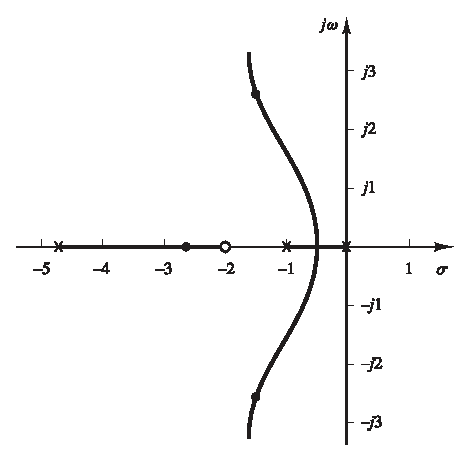
\includegraphics[width=5cm]{images/ejemplo1_LGRcompensado.eps}
			\end{figure}
		\end{column}
	\end{columns}
	\pause
	El polo ubicado en $s=-2.65$ está muy cerca del cero en $s=-1.9432$, por lo cual su influencia en el transitorio es mínima.
\end{frame}

\begin{frame}[c]\frametitle{Procedimiento de Diseño Compensador en Adelanto usando LGR - Ejemplo}
	\begin{figure}
		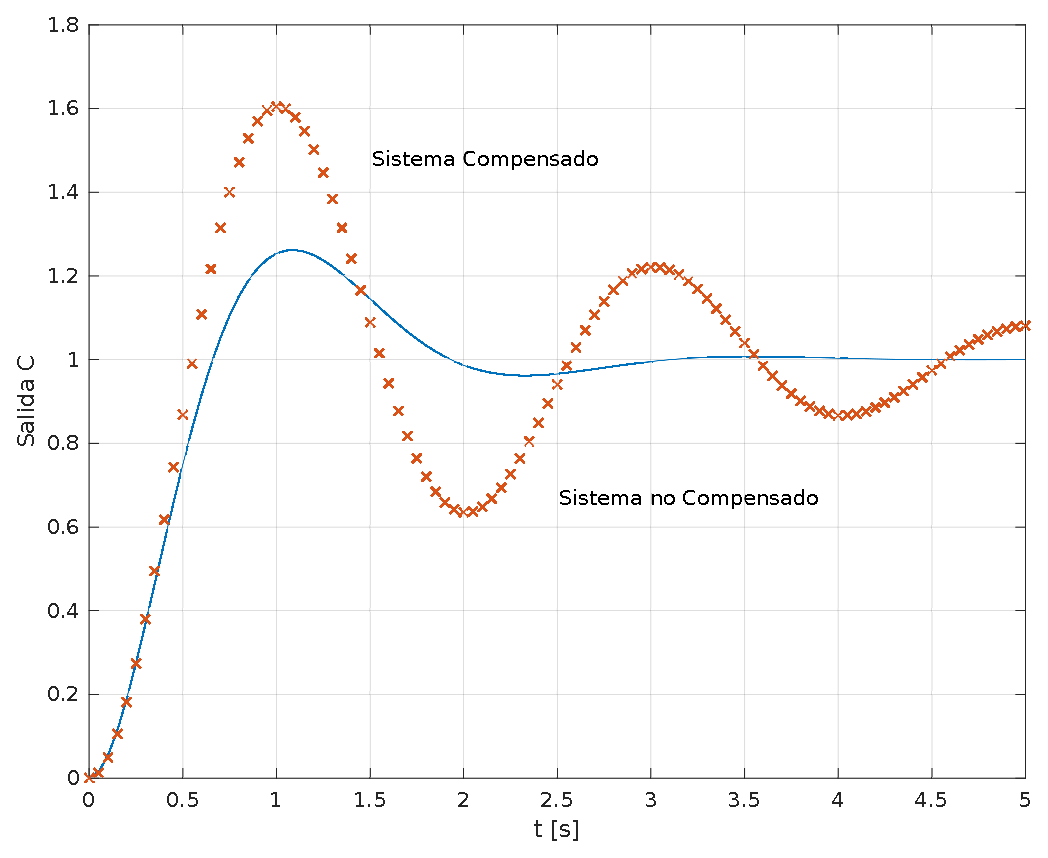
\includegraphics[width=8cm]{images/ejemplo1_comparacion.eps}
	\end{figure}
	\vspace*{-4mm}
	\centering \small Respuesta paso del Sistema no Compensado y Compensado
\end{frame}

\begin{frame}[c]\frametitle{Procedimiento de Diseño Compensador en Adelanto usando LGR - Ejemplo}
	\begin{figure}
		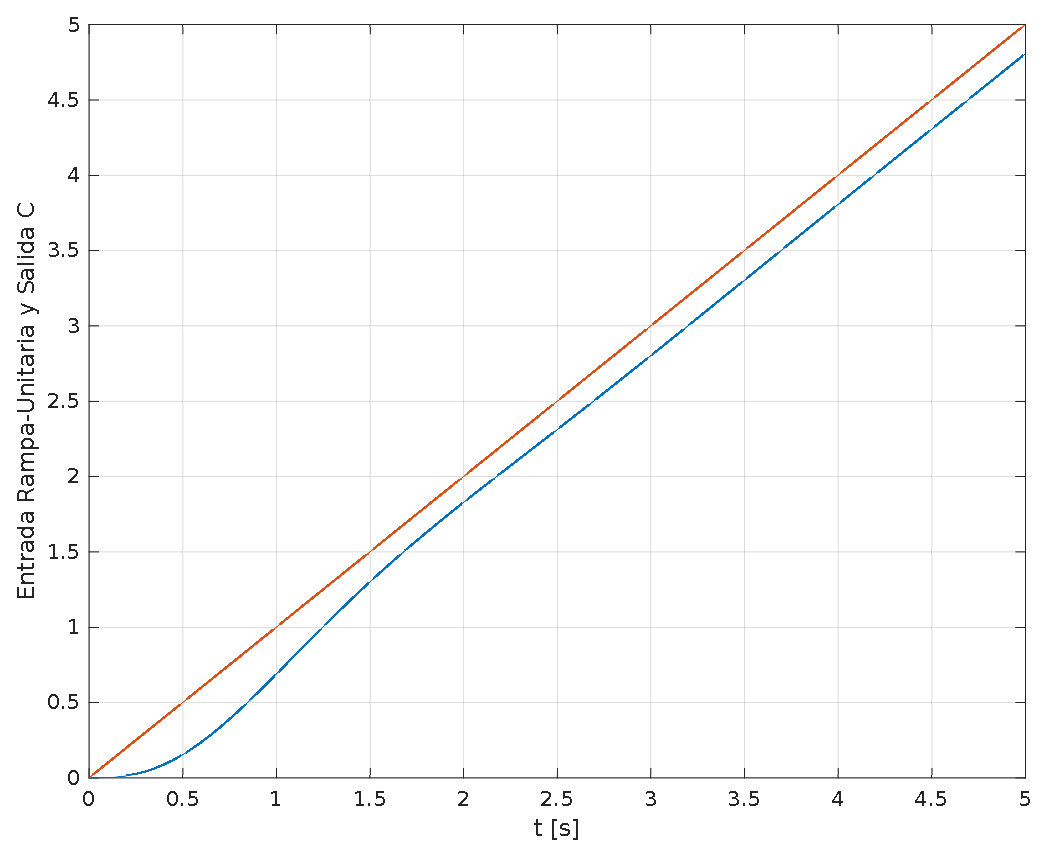
\includegraphics[width=8cm]{images/ejemplo1_comparacion_rampa.eps}
	\end{figure}
	\vspace*{-4mm}
	\centering \small Respuesta Rampa del Sistema Compensado
\end{frame}

\section{Compensación en Atraso}
\begin{frame}[<+->]\frametitle{Compensación en Atraso}
	\begin{itemize}
		\item Considere el problema de encontrar un compensador cuando el sistema tiene una respuesta transitoria satisfactoria pero características de estado estacionario insatisfactorias.
		\item Compensación $\rightarrow$ aumentar la ganancia de lazo abierto sin cambiar de forma notoria las características de la respuesta transitoria.
		\item El LGR en las cercanías a los polos dominantes no debería cambiar significativamente.
		\item La contribución del ángulo del compensador en atraso debe limitarse a un valor pequeño (p. ej. $-\ang{5} < \phi_{lag} < 0$). Para lograrlo se ubican un polo y un cero cercanos entre si y cercanos al origen.
	\end{itemize}
\end{frame}

\begin{frame}[<+->]\frametitle{Procedimiento de Diseño para el Compensador en Atraso usando LGR}
	\begin{enumerate}
		\item Dibujar el LGR para el sistema no compensado. Con base en los requerimientos de la respuesta transitoria, localice los polos dominantes de lazo cerrado en el LGR.
		\item Asuma un compensador en atraso de la forma:
		\begin{equation*}
			G_c(s) = \hat{K}_c \frac{s+\frac{1}{T}}{s+\frac{1}{\beta T}}
		\end{equation*}
		\item Evaluar la constante de error estático especificada por el problema.
		\item Determine el incremento necesario en la constante de error estático para satisfacer los requerimientos.
		\item Determine el polo y cero del compensador que produce el incremento necesario en la constante de error estático sin alterar apreciablemente el LGR original.
		\seti
	\end{enumerate}
\end{frame}

\begin{frame}[<+->]\frametitle{Procedimiento de Diseño para el Compensador en Atraso usando LGR}
	\begin{enumerate}
		\conti
		\item Dibujar un nuevo LGR para el sistema compensado. Localice los polos dominantes de lazo cerrado deseados. Si la contribución de ángulo del compensador es muy pequeña, el LGR debería ser casi idéntico. Ubique en el nuevo LGR los polos de lazo cerrado deseados de acuerdo con las especificaciones de la respuesta transitoria.
		\item Ajustar la ganancia $\hat{K}_c$ del compensador usando la condición de magnitud para que los polos dominantes estén en la ubicación deseada. El valor de $\hat{K}_c$ será aproximadamente 1.
	\end{enumerate}
\end{frame}


\begin{frame}[c]\frametitle{Procedimiento de Diseño Compensador en Adelanto usando LGR - Ejemplo}
\begin{columns}
	\begin{column}{0.4\textwidth}
		\begin{figure}
			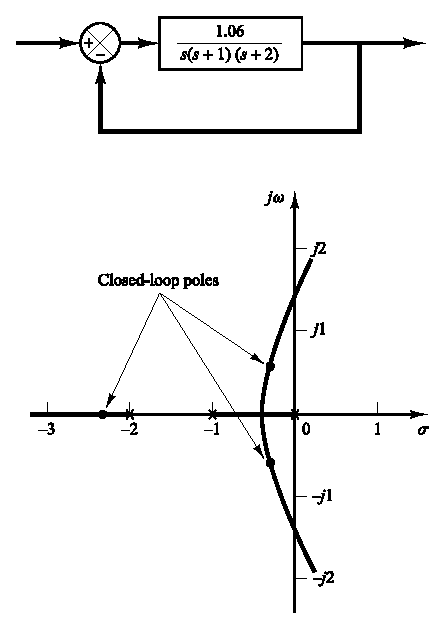
\includegraphics[width=4.5cm]{images/ejemplo2_planta.eps}
		\end{figure}
	\end{column}
	\begin{column}{0.6\textwidth}
		Considere el sistema mostrado en la figura. La función de transferencia de la planta es:
		\begin{equation*}
			G(s) = \frac{1.06}{s(s+1)(s+2)}
		\end{equation*}
		\pause	
		Los polos dominantes de lazo cerrado son $s = -0.3307 \pm j0.5864$. El factor de amortiguamiento es $\zeta = 0.491$. La frecuencia natural es $\omega_n = 0.673$ rad/s. La constante de error estático de velocidad es $0.53\ s^{-1}$.
	\end{column}
\end{columns}
\end{frame}

\begin{frame}[c]\frametitle{Procedimiento de Diseño Compensador en Adelanto usando LGR - Ejemplo}
\begin{columns}
	\begin{column}{0.5\textwidth}
		Se desea aumentar la constante de error estático de velocidad $K_v$ a un valor de $5\ s^{-1}$ sin afectar la ubicación de los polos dominantes. Para lograrlo se introduce un compensador en atraso.\\
		\vspace*{3mm}
		\pause
		Para incrementar la constante de error estático de velocidad en un factor de 10, se selecciona $\beta = 10$, y se ubican el cero y el polo del compensador en $s=-0.05$ y $s=-0.005$, respectivamente.
		\pause
	\end{column}
	\begin{column}{0.5\textwidth}
		La función de transferencia del compensador en atraso queda:
		\begin{equation*}
			G_c(s) = \hat{K}_c \frac{s+0.05}{s+0.005}
		\end{equation*}
		\pause
		La contribución de ángulo del compensador sobre un polo dominante es:
		\begin{align*}
			\angle G_c(s) &= \angle(s+0.05) - \angle(s+0.005)\\
			&= \ang{115.5797} - \ang{119.0488} = -\ang{3.4691}
		\end{align*}
	\end{column}
\end{columns}
\end{frame}

\begin{frame}[c]\frametitle{Procedimiento de Diseño Compensador en Adelanto usando LGR - Ejemplo}
La función de transferencia de lazo abierto del sistema compensado es:
\begin{align*}
	G_c(s)G(s) &= \hat{K}_c \frac{s+0.05}{s+0.005} \frac{1.06}{s(s+1)(s+2)}\\
	&= \frac{K(s+0.05)}{s(s+0.005)(s+1)(s+2)}
\end{align*}
donde $K = 1.06 \hat{K}_c$.
\end{frame}

\begin{frame}[c]\frametitle{Procedimiento de Diseño Compensador en Adelanto usando LGR - Ejemplo}
	\begin{figure}
		\centering
		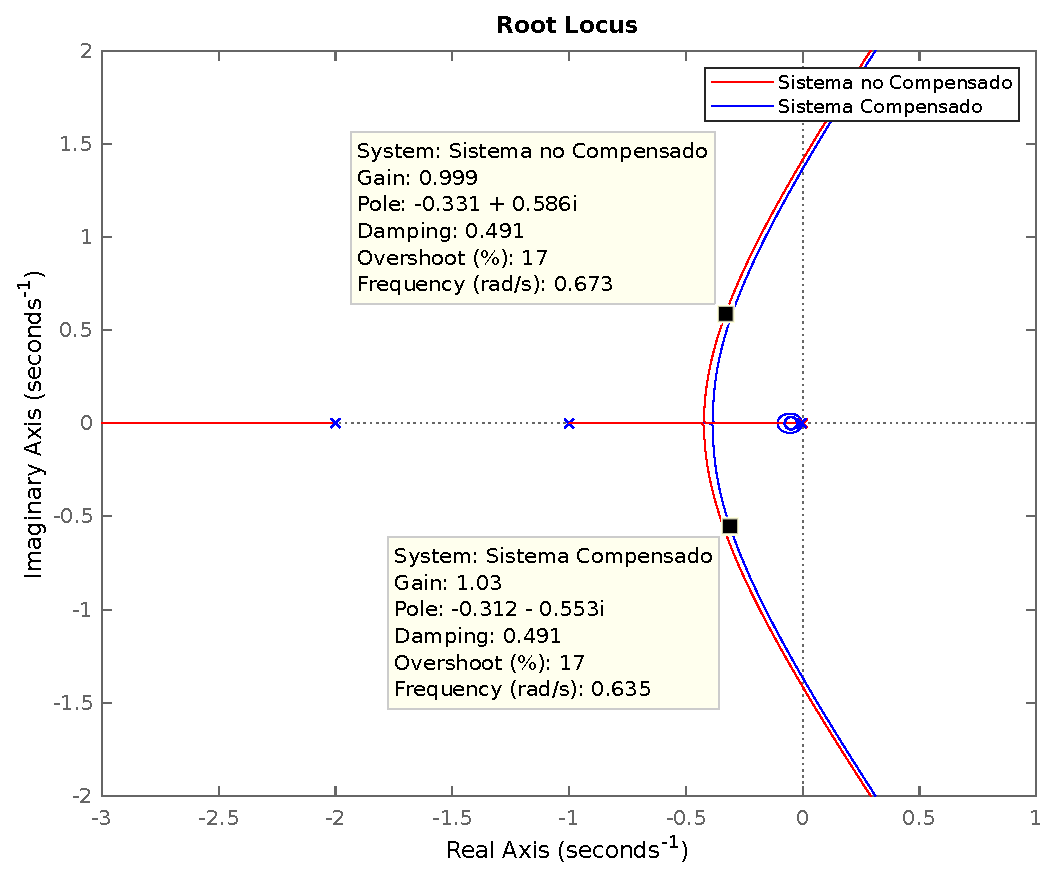
\includegraphics[width=8cm]{images/ejemplo2_LGRcompensado.eps}
	\end{figure}
	\vspace*{-5mm}
	\centering \small Comparación de LGR sistema no compensado y sistema compensado.
\end{frame}

\begin{frame}[c]\frametitle{Procedimiento de Diseño Compensador en Adelanto usando LGR - Ejemplo}
	\begin{figure}
		\centering
		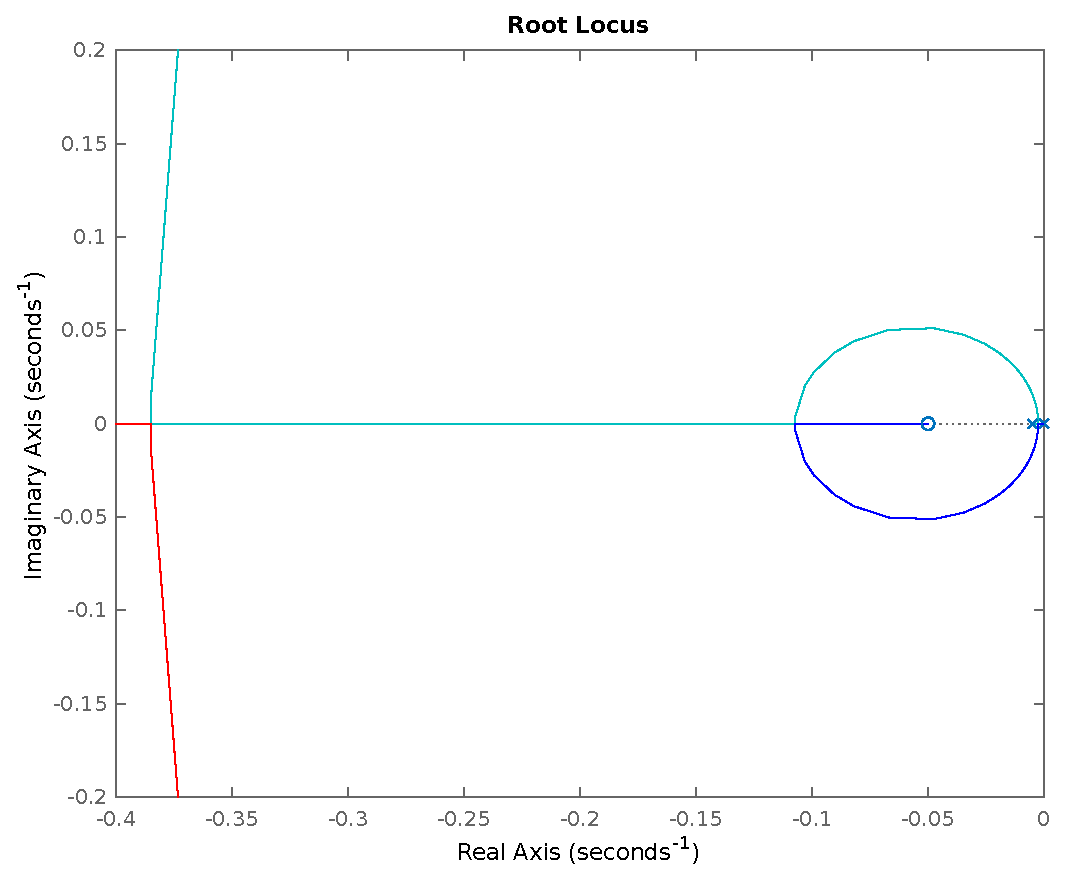
\includegraphics[width=8cm]{images/ejemplo2_LGR_origen.eps}
	\end{figure}
	\vspace*{-5mm}
	\centering \small Lugar de las raíces en cercanías al origen.
\end{frame}

\begin{frame}[c]\frametitle{Procedimiento de Diseño Compensador en Adelanto usando LGR - Ejemplo}
	\small
	\vspace*{3mm}
	\begin{columns}
		\begin{column}{0.5\textwidth}
			La ganancia $K$ de lazo abierto se determina usando la condición de magnitud:
			\begin{align*}
				K &= \left| \frac{s(s+0.005)(s+1)(s+2)}{s+0.05} \right|_{s=-0.31+j0.55}\\
				&= 1.0235
			\end{align*}
			\pause
			La ganancia del compensador se obtiene como:
			\begin{equation*}
				\hat{K}_c = \frac{K}{1.06} = \frac{1.0235}{1.06} = 0.9656
			\end{equation*}
			\pause
		\end{column}
		\begin{column}{0.5\textwidth}
			Función de transferencia del compensador en atraso:
			\begin{equation*}
				G_c(s) = 0.9656\frac{s+0.05}{s+0.005} = 9.656\frac{20s+1}{200s+1}
			\end{equation*}
			\pause
			Función de transferencia de lazo abierto del sistema compensado:
			\begin{align*}
				G_c(s)G(s) &= \frac{1.0235(s+0.05)}{s(s+0.005)(s+1)(s+2)}\\
				&= \frac{5.12(20s+1)}{s(200s+1)(s+1)(0.5s+1)}
			\end{align*}
			\pause
			Constante de error estático de velocidad:
			\begin{equation*}
				K_v = \lim_{s \rightarrow 0}sG_c(s)G(s) = 5.12 s^{-1}
			\end{equation*}
		\end{column}
	\end{columns}
\end{frame}

\begin{frame}[<+->]\frametitle{Procedimiento de Diseño Compensador en Adelanto usando LGR - Ejemplo}
	\begin{itemize}
		\item Polo y cero localizados cerca del origen $\rightarrow$ efecto pequeño en la forma del LGR.
		\item El valor de la constante de error de velocidad estático aumentó aproximadamente 10 veces!
		\item El par polo y cero agregados genera una \textit{cola larga} de pequeña amplitud en el transitorio.
		\item La respuesta del sistema compensado es más lenta que la del sistema original.
	\end{itemize}
\end{frame}

\begin{frame}[<+->]\frametitle{Procedimiento de Diseño Compensador en Adelanto usando LGR - Ejemplo}
\begin{figure}
	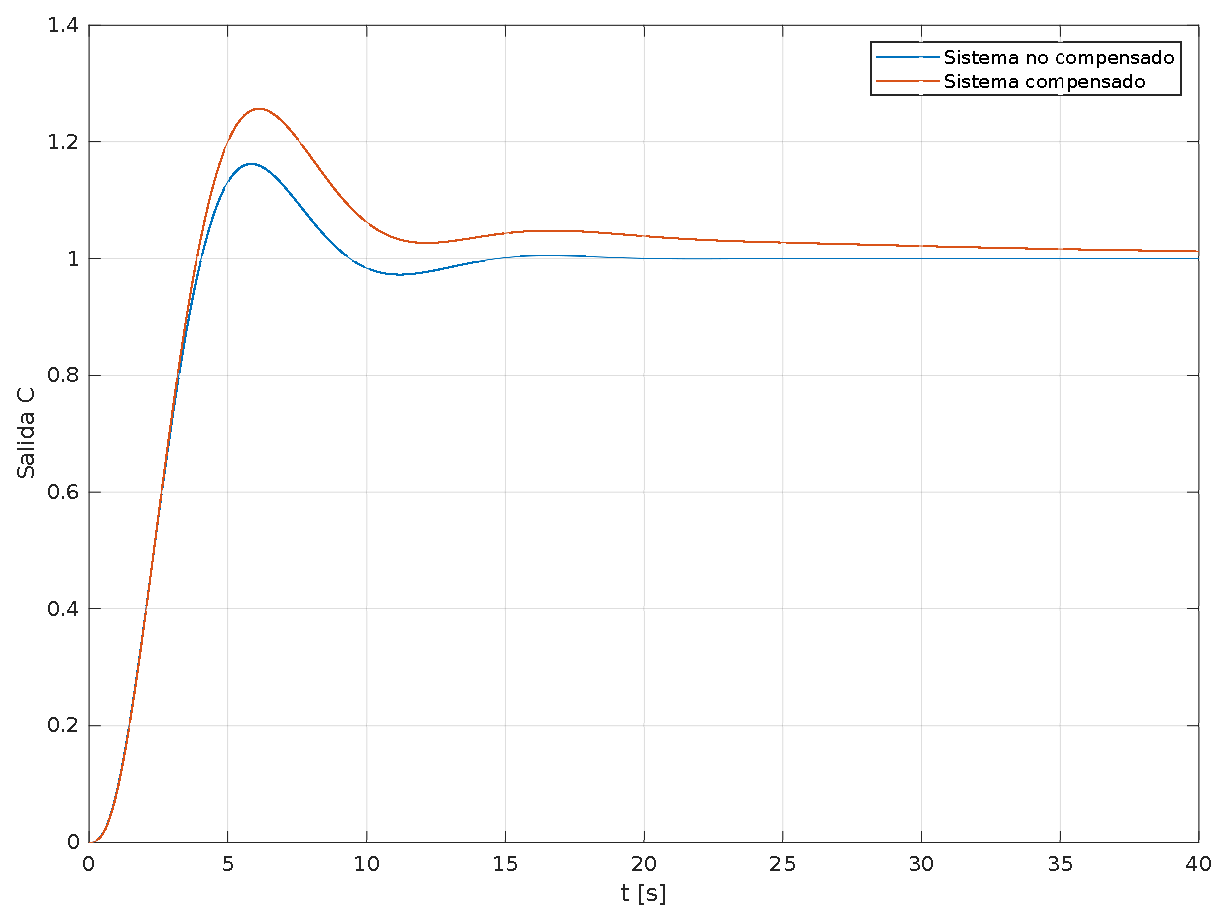
\includegraphics[width=8.5cm]{images/ejemplo2_comparacion_paso.eps}
\end{figure}
\vspace*{-3mm}
\centering \small Respuesta ante paso unitario para sistema no compensado y sistema compensado.
\end{frame}

\begin{frame}[<+->]\frametitle{Procedimiento de Diseño Compensador en Adelanto usando LGR - Ejemplo}
\begin{figure}
	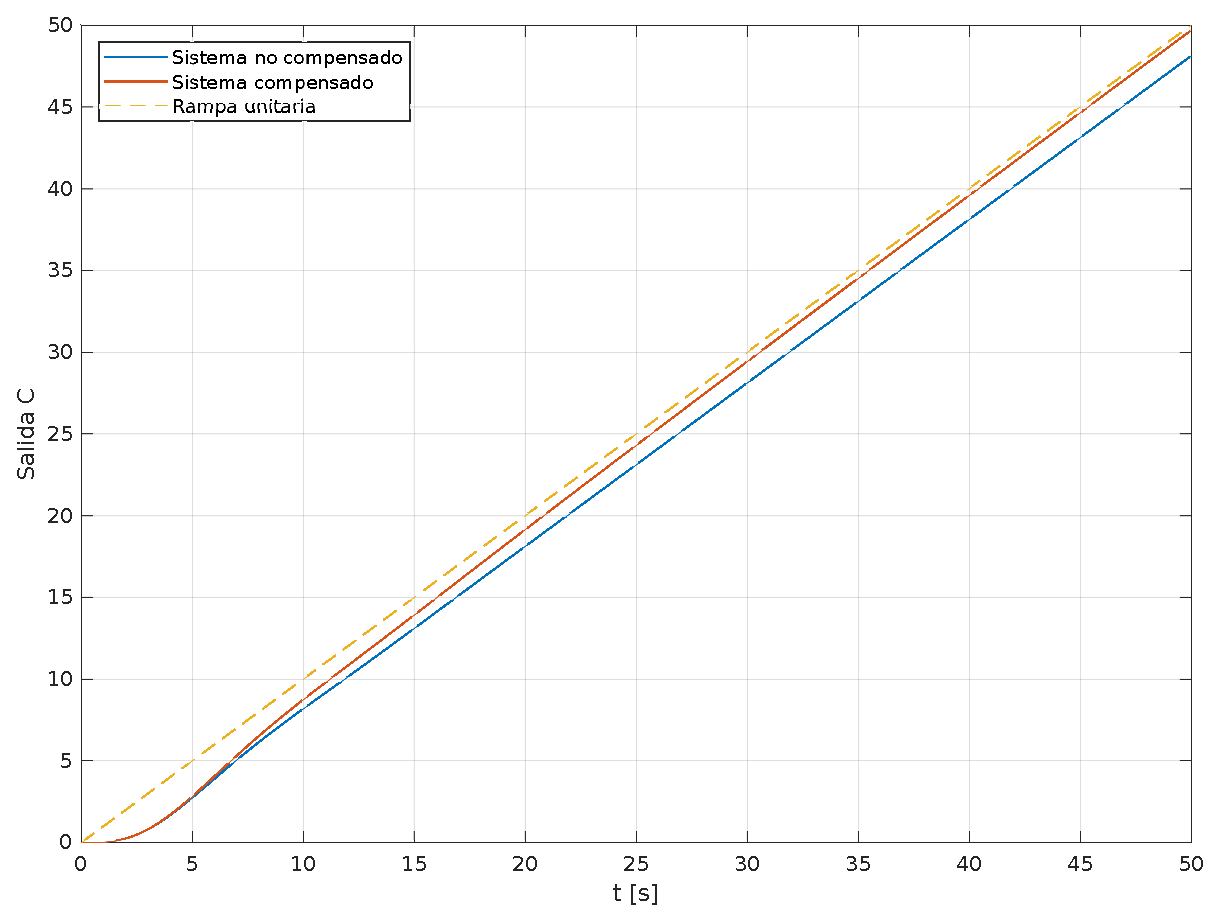
\includegraphics[width=8.5cm]{images/ejemplo2_comparacion_rampa.eps}
\end{figure}
\vspace*{-3mm}
\centering \small Respuesta ante rampa unitaria para sistema no compensado y sistema compensado.
\end{frame}

\section{Compensación Adelanto - Atraso}
\begin{frame}[<+->]\frametitle{Compensación Adelanto - Atraso}
	\begin{itemize}
		\item Compensación en adelanto: aumenta la velocidad de respuesta, aumenta la estabilidad del sistema.
		\item Compensación en atraso: mejora la exactitud del sistema en estado estacionario, reduce la velocidad de respuesta.
		\item Si se desea mejorar tanto la respuesta transitoria como la estacionaria, se puede utilizar simultaneamente un compensador en adelanto y uno en atraso $\rightarrow$ compensador de adelanto-atraso
	\end{itemize}
\end{frame}

\begin{frame}[<+->]\frametitle{Procedimiento de Diseño para el Compensador en Adelanto-Atraso usando LGR}
	Asumiendo un compensador en adelanto-atraso de la forma:
	\begin{equation*}
		G_c(s) = K_c \frac{\beta}{\gamma} \frac{(T_1 s + 1)(T_2 s + 1)}{(\frac{T_1}{\gamma} s + 1)(\beta T_2 s + 1)} = K_c \left( \frac{s+\frac{1}{T_1}}{s+\frac{\gamma}{T_1}} \right)\left( \frac{s+\frac{1}{T_2}}{s+\frac{1}{\beta T_2}} \right)
	\end{equation*}
	donde $\beta > 1$ y $\gamma > 1$. Considere que $K_c$ pertenece a la parte de adelanto del compensador.
\end{frame}

\begin{frame}[<+->]\frametitle{Procedimiento de Diseño para el Compensador en Adelanto-Atraso usando LGR}
\small
Caso 1: $\gamma \neq \beta$ $\rightarrow$ El proceso de diseño es una combinación del diseño de un compensador en adelanto y uno de atraso.
\pause
	\begin{enumerate}
		\item A partir de las especificaciones de desempeño, determine la ubicación deseada para los polos dominantes de lazo cerrado.
		\item Usando la función de transferencia del sistema no compensado $G(s)$, determine el ángulo faltante $\phi$. El compensador en adelanto debe contribuir dicho ángulo $\phi$.
		\seti
	\end{enumerate}
\end{frame}

\begin{frame}[<+->]\frametitle{Procedimiento de Diseño para el Compensador en Adelanto-Atraso usando LGR}
\small
	\begin{enumerate}
		\conti
		\item Asumiendo que más adelante se seleccionará $T_2$ suficientemente grande tal que la magnitud de la parte de atraso es aproximadamente la unidad, seleccione los valores de $T_1$ y $\gamma$ tal que:
		\begin{equation*}
			\angle\left(\frac{s_1+\frac{1}{T_1}}{s_1+\frac{\gamma}{T_1}} \right) = \phi
		\end{equation*}
		donde $s = s_1$ es uno de los polos dominantes. La selección de $T_1$ y $\gamma$ no es única.
		\pause
		Luego determine el valor de $K_c$ de la condición de magnitud:
		\begin{equation*}
			\left| K_c \frac{s_1+\frac{1}{T_1}}{s_1+\frac{\gamma}{T_1}} G(s_1) \right| = 1
		\end{equation*}
		\seti
	\end{enumerate}
\end{frame}

\begin{frame}[<+->]\frametitle{Procedimiento de Diseño para el Compensador en Adelanto-Atraso usando LGR}
\small
\begin{columns}
	\begin{column}{0.6\textwidth}
	\begin{enumerate}
		\conti
		\item Si la constante de error de velocidad estática $K_v$ ha sido especificada, determine el valor de $\beta$ para satisfacer dicho requerimiento.
		\pause
		La constante de error de velocidad estática $K_v$ está dada por:
		\begin{align*}
			K_v &= \lim_{s \rightarrow 0} s G_c(s)G(s)\\
			&= \lim_{s \rightarrow 0} s K_c \left( \frac{s+\frac{1}{T_1}}{s+\frac{\gamma}{T_1}} \right)\left( \frac{s+\frac{1}{T_2}}{s+\frac{1}{\beta T_2}} \right) G(s)\\
			&= \lim_{s \rightarrow 0} s K_c \frac{\beta}{\gamma} G(s)
		\end{align*}
		donde $K_c$ y $\gamma$ ya han sido deteminados en el paso 3. 
	\end{enumerate}
	\end{column}
	\begin{column}{0.4\textwidth}
	\pause
	Tomando el valor de $K_v$ se puede obtener el valor de $\beta$. Con dicho valor de $\beta$ se selecciona $T_2$ tal que
	\begin{align*}
		&\left| \frac{s_1+\frac{1}{T_2}}{s_1+\frac{1}{\beta T_2}} \right| \approx 1\\
		-\ang{5} < \angle&\left( \frac{s_1+\frac{1}{T_2}}{s_1+\frac{1}{\beta T_2}} \right) < \ang{0}
	\end{align*}
	\end{column}
\end{columns}
\end{frame}

\begin{frame}[<+->]\frametitle{Procedimiento Diseño Compensador en Adelanto-Atraso usando LGR - Ejemplo}
\begin{columns}
	\begin{column}{0.5\textwidth}
		\begin{figure}
			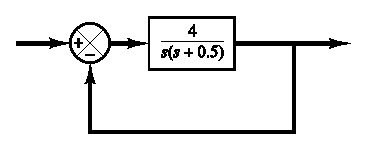
\includegraphics[width=4cm]{images/ejemplo3_planta.eps}
		\end{figure}
		Considere el sistema de control de la figura. La función de transferencia de la planta es:
		\begin{equation*}
			G(s) = \frac{4}{s(s+0.5)}
		\end{equation*}
	\end{column}
	\begin{column}{0.5\textwidth}
		Los polos del sistema en lazo cerrado son $s = -0.25 \pm j1.9843$. En este caso $\zeta = 0.125$, $\omega_n = 2$ y $K_v = 8$.\\
		\vspace*{3mm}
		\pause
		El desempeño deseado es $\zeta = 0.5$, $\omega_n = 5$, $K_v = 80$. Se debe diseñar un compensador apropiado para satisfacer todos los requerimientos.
	\end{column}
\end{columns}
\end{frame}

\begin{frame}[<+->]\frametitle{Procedimiento Diseño Compensador en Adelanto-Atraso usando LGR - Ejemplo}
	Se asume que el compensador tiene la forma
	\begin{equation*}
		G_c(s) = K_c \left( \frac{s+\frac{1}{T_1}}{s+\frac{\gamma}{T_1}} \right)\left( \frac{s+\frac{1}{T_2}}{s+\frac{1}{\beta T_2}} \right),\ \beta > 1,\ \gamma > 1,\ \gamma \neq \beta
	\end{equation*}
	\pause
	A partir de las especificaciones, los polos dominantes de lazo cerrado deseados son $s = -2.5 \pm j4.33$.\\
	\vspace*{3mm}
	\pause
	El ángulo del sistema no compensado es:	
	\begin{equation*}
		\angle\left.\frac{4}{s(s+0.5)}\right|_{s=-2.5 \pm j4.33} = -\ang{120} -\ang{114.7919} = -\ang{234.7926} = \ang{125.2074}
	\end{equation*}
	\pause
	El ángulo faltante $\phi$ que debe contribuir la parte de adelanto es:
	\begin{equation*}
		\phi = \ang{180} - \ang{125.2074} = \ang{54.7926}
	\end{equation*}
\end{frame}

\begin{frame}[<+->]\frametitle{Procedimiento Diseño Compensador en Adelanto-Atraso usando LGR - Ejemplo}
	Se procede a determinar la ubicación del cero y polo que contribuyen el ángulo $\phi$. En éste caso se decide ubicar el cero en $s=-0.5$ para que se cancele con el polo de la planta en $s = -0.5$.\\
	\vspace*{3mm}
	\pause
	Con ésta ubicación del cero, se calcula que el polo debe estar ubicado en $s = -5.02$ para contribuir el ángulo $\phi$.\\
	\vspace*{3mm}
	\pause
	Entonces, la parte de adelanto del compensador será:
	\begin{equation*}
		K_c\frac{s+\frac{1}{T_1}}{s+\frac{\gamma}{T_1}} = K_c\frac{s+0.5}{s+5.02}
	\end{equation*}
	\vspace*{3mm}
	\pause
	Por lo tanto, $T_1 = 2$, $\gamma = \frac{5.02}{0.5} = 10.04$.
\end{frame}

\begin{frame}[<+->]\frametitle{Procedimiento Diseño Compensador en Adelanto-Atraso usando LGR - Ejemplo}
	El valor de $K_c$ se determina de la condición de magnitud:
	\begin{equation*}
		\left| K_c \frac{s+0.5}{s+5.02} \frac{4}{s(s+0.5)} \right|_{s=-2.5+j4.33} = 1
	\end{equation*}
	\begin{equation*}
		K_c = \left| \frac{(s+5.02)s}{4} \right|_{s=-2.5+j4.33} = 6.26
	\end{equation*}
\end{frame}

\begin{frame}[<+->]\frametitle{Procedimiento Diseño Compensador en Adelanto-Atraso usando LGR - Ejemplo}
	Ahora se procede a diseñar la parte de atraso del compensador. Primero se determina el valor de $\beta$ para satisfacer el requerimiento de constante de error de velocidad estática:
	\begin{align*}
		K_v &= \lim_{s \rightarrow 0} sG_c(s)G(s)\\
		&= \lim_{s \rightarrow 0}s K_c \frac{\beta}{\gamma}G(s)\\
		&= \lim_{s \rightarrow 0} s (6.26) \frac{\beta}{10.04}\frac{4}{s(s+0.5)} = 4.988\beta = 80\\
		\Rightarrow \beta &= 16.04
	\end{align*}
\end{frame}

\begin{frame}[<+->]\frametitle{Procedimiento Diseño Compensador en Adelanto-Atraso usando LGR - Ejemplo}
	Finalmente, se selecciona el valor de $T_2$ tal que las siguientes condiciones sean satisfechas:
	\begin{equation*}
		\left| \frac{s+\frac{1}{T_2}}{s+\frac{1}{16.04 T_2}} \right|_{s=-2.5 + j4.33} \approx 1, \hspace{1cm}
		-\ang{5} < \angle\left.\left( \frac{s+\frac{1}{T_2}}{s+\frac{1}{\beta T_2}} \right) \right|_{s=-2.5 + j4.33} < \ang{0}
	\end{equation*}
	\pause
	Se pueden seleccionar varios valores de $T_2$ y verificar si las condiciones se satisfacen. Tomando $T_2 = 5$ se encuentra que:
	\begin{equation*}
		0.98 < \text{magnitud} < 1, \hspace*{1cm} -\ang{2.10} < \text{ángulo} < \ang{0}
	\end{equation*}
	\pause
	Como se satisfacen ambas condiciones, se selecciona $T_2 = 5$.
\end{frame}

\begin{frame}[<+->]\frametitle{Procedimiento Diseño Compensador en Adelanto-Atraso usando LGR - Ejemplo}
	La función de transferencia del compensador adelanto-atraso diseñado es:
	\begin{align*}
		G_c(s) &= 6.26 \left( \frac{s+\frac{1}{2}}{s+\frac{10.04}{2}} \right) \left( \frac{s+\frac{1}{5}}{s+\frac{1}{(16.04)(5)}} \right)\\
		&= 6.26\left( \frac{s+0.5}{s+5.02} \right)\left( \frac{s+0.2}{s+0.01247} \right)\\
		&= \frac{10(2s+1)(5s+1)}{(0.1992s+1)(80.19s+1)}
	\end{align*}
	\pause
	La función de transferencia de lazo abierto del sistema compensado es:
	\begin{equation*}
		G_c(s)G(s) = \frac{25.04(s+0.2)}{s(s+50.2)(s+0.01247)}
	\end{equation*}
	\pause
	Debido a la cancelación polo-cero, el sistema compensado es de tercer orden.
\end{frame}

\begin{frame}[<+->]\frametitle{Procedimiento Diseño Compensador en Adelanto-Atraso usando LGR - Ejemplo}
\begin{columns}
	\begin{column}{0.5\textwidth}
		\begin{figure}
			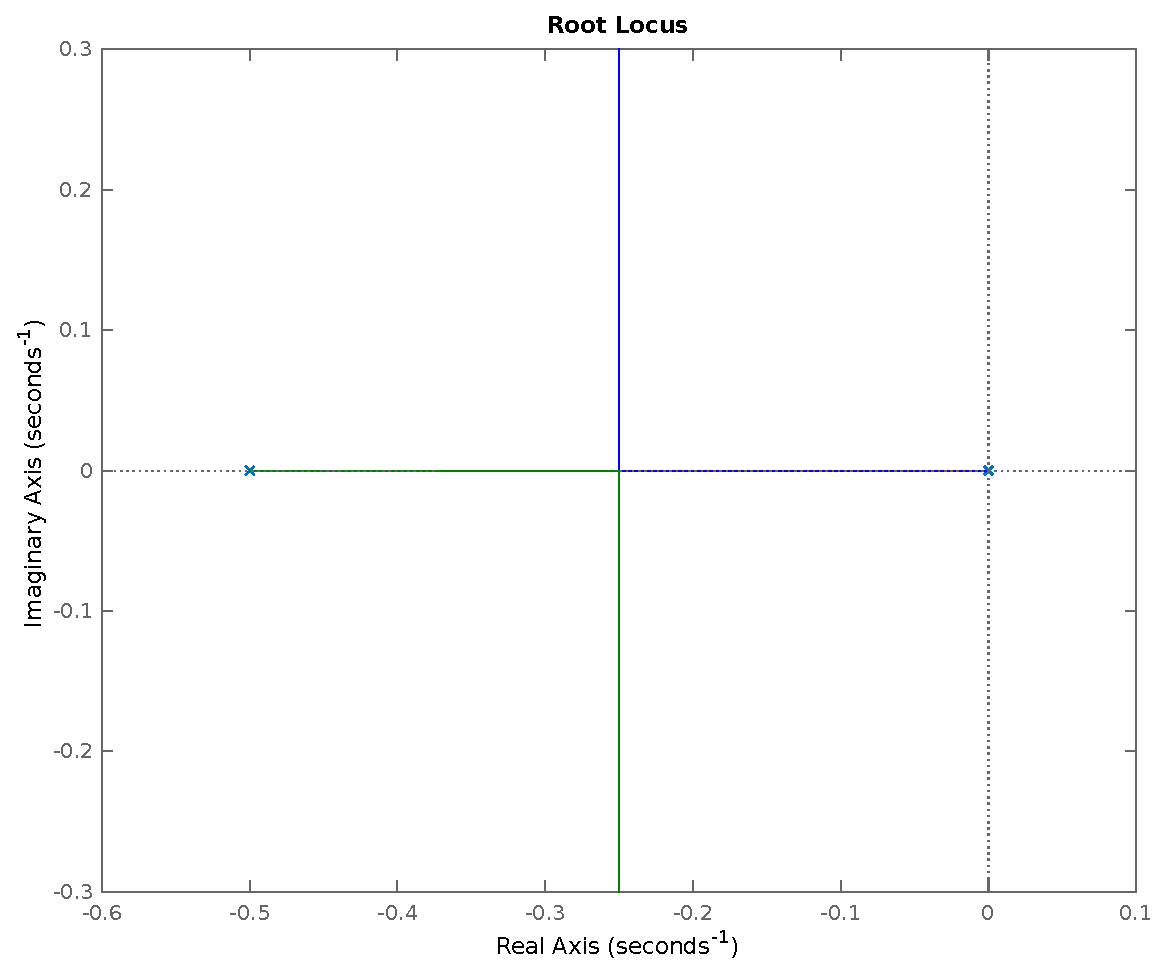
\includegraphics[width=7cm]{images/ejemplo3_LGR_uncomp.eps}
		\end{figure}
		\centering \small LGR para el sistema no compensado
	\end{column}
	\begin{column}{0.5\textwidth}
		\begin{figure}
			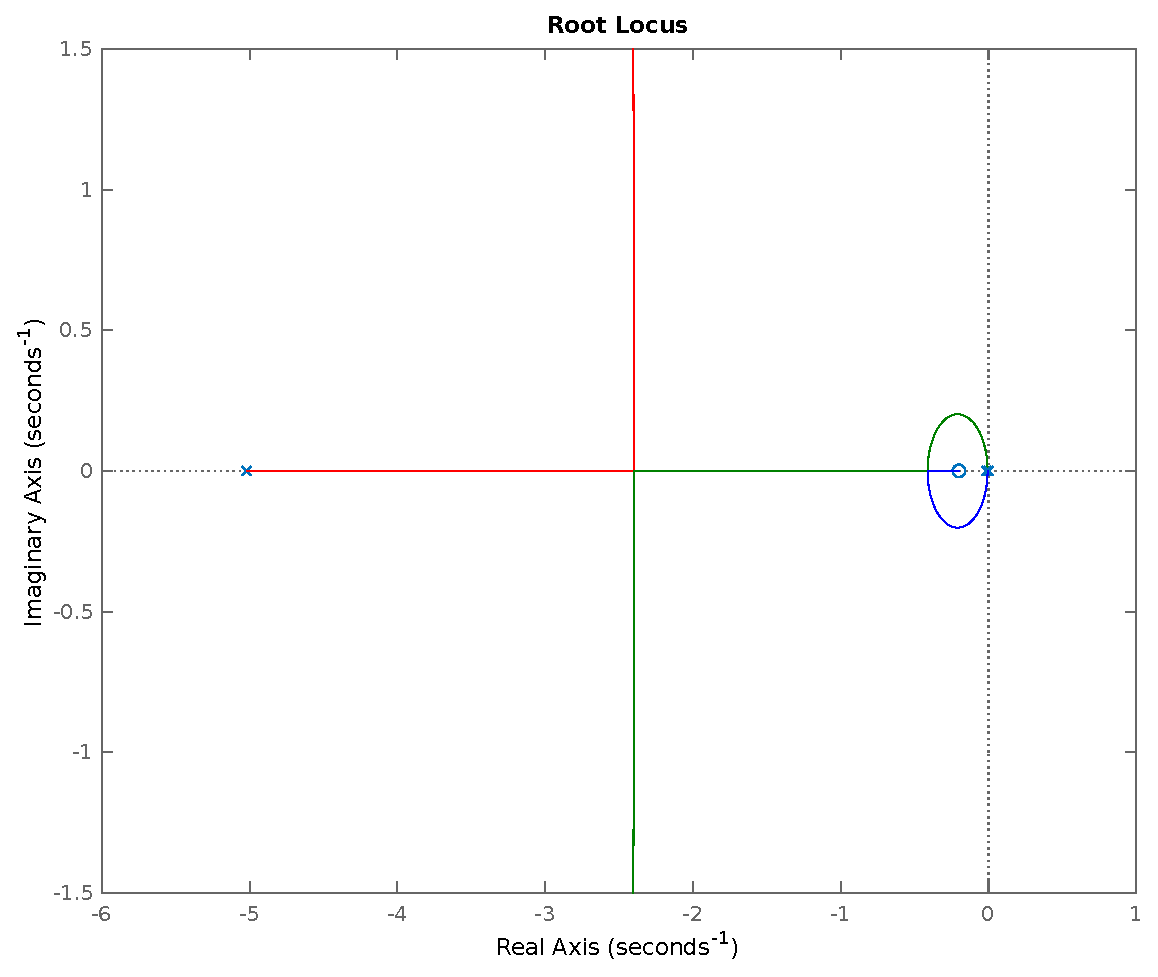
\includegraphics[width=7cm]{images/ejemplo3_LGR_comp.eps}
		\end{figure}
		\centering \small LGR para el sistema compensado
	\end{column}
\end{columns}	
\end{frame}

\begin{frame}[<+->]\frametitle{Procedimiento Diseño Compensador en Adelanto-Atraso usando LGR - Ejemplo}
	\begin{figure}
		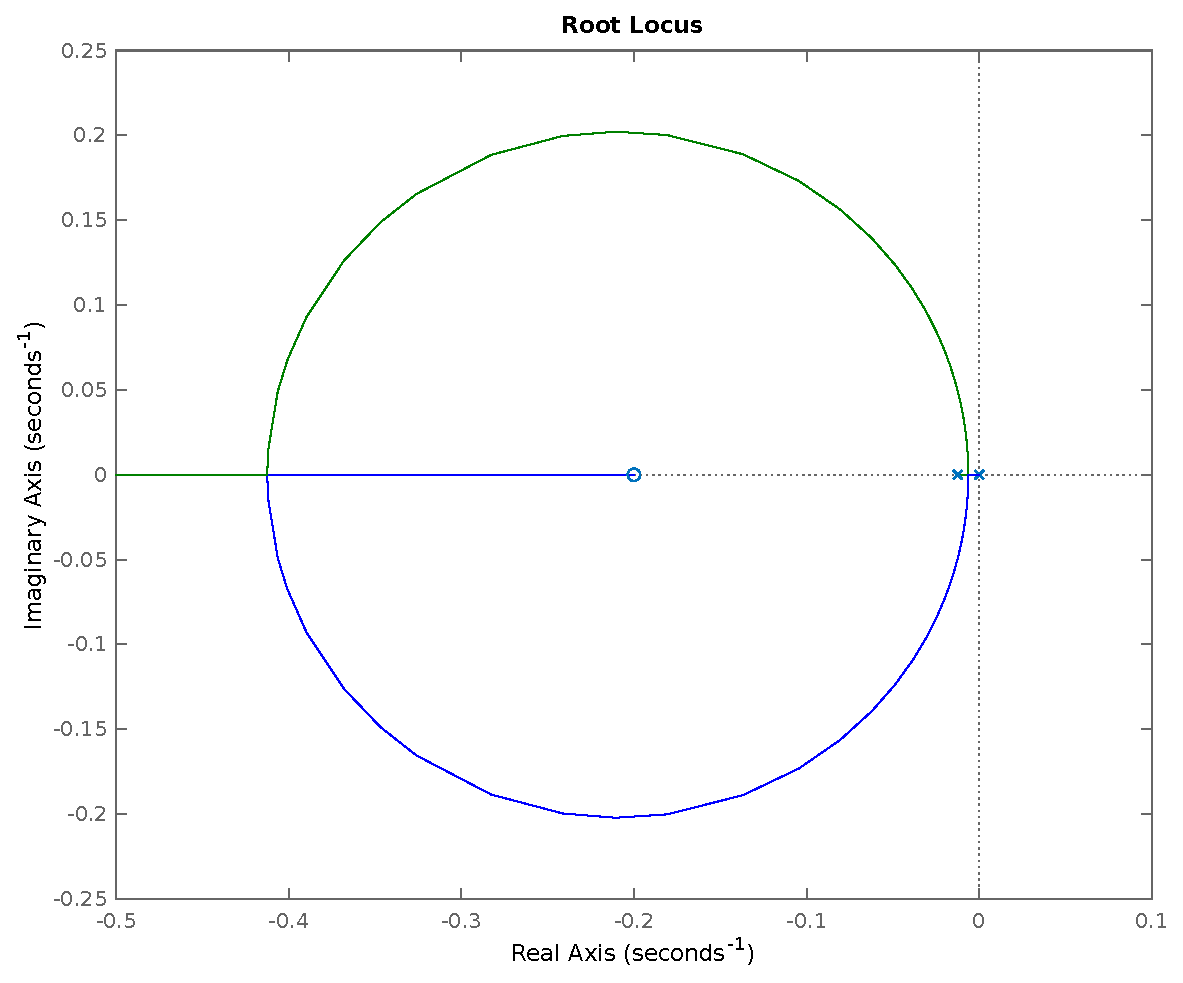
\includegraphics[width=7cm]{images/ejemplo3_LGR_comp_detalle.eps}
	\end{figure}
	\centering \small LGR para el sistema compensado - detalle cerca del origen
\end{frame}

\begin{frame}[<+->]\frametitle{Procedimiento Diseño Compensador en Adelanto-Atraso usando LGR - Ejemplo}
	\begin{figure}
		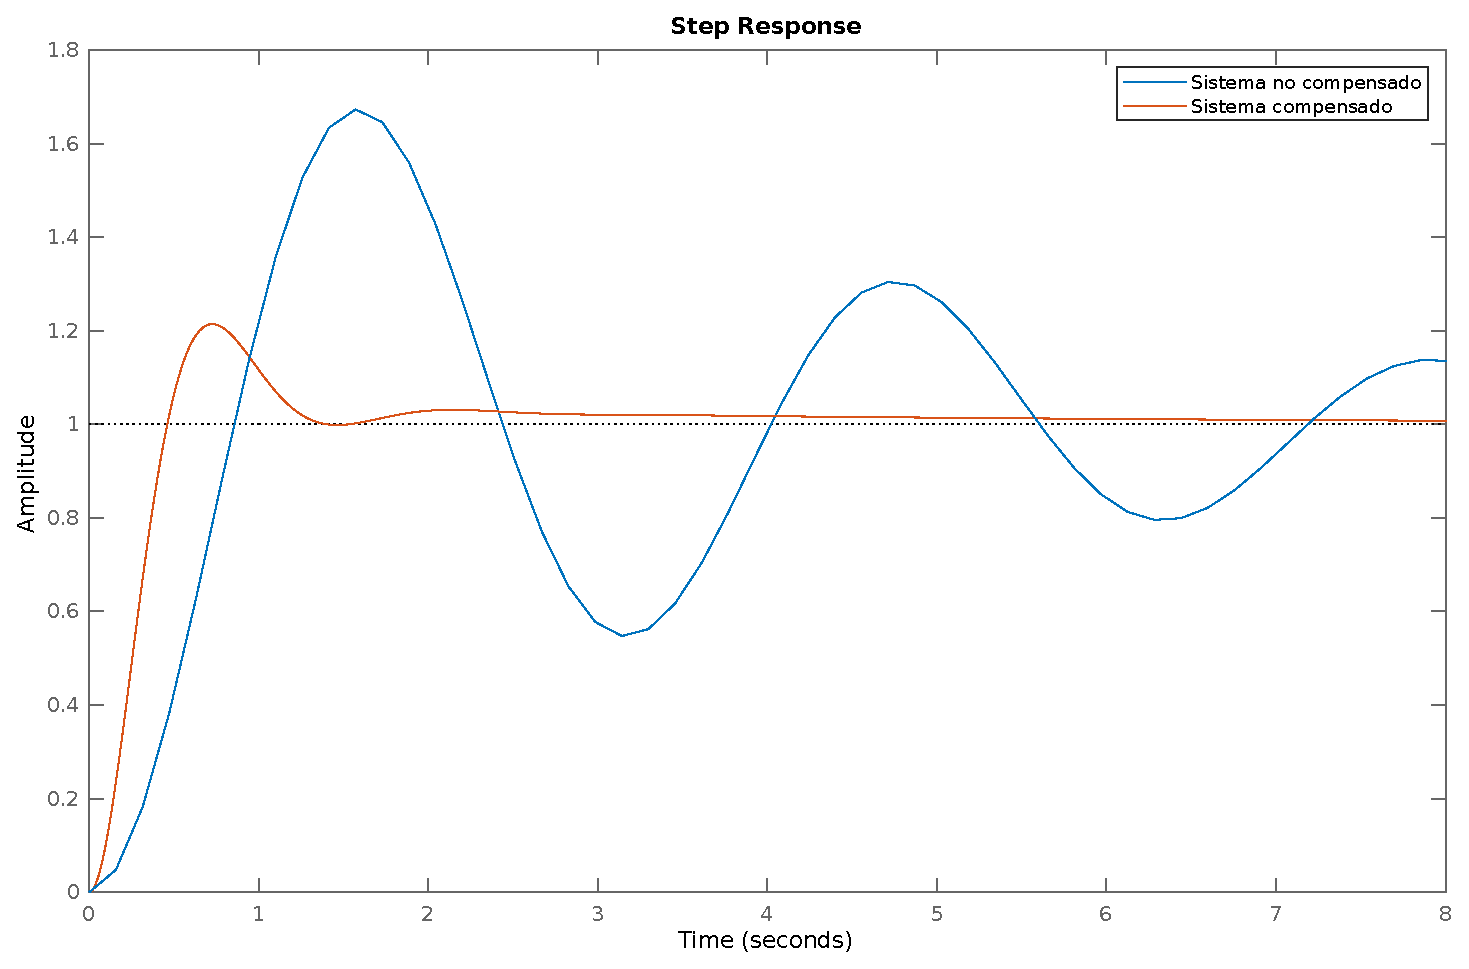
\includegraphics[width=10cm]{images/ejemplo3_comparacion_paso.eps}
	\end{figure}
	\vspace*{-5mm}
	\centering \footnotesize Respuesta paso para sistema no compensado y compensado
\end{frame}

\begin{frame}[<+->]\frametitle{Procedimiento Diseño Compensador en Adelanto-Atraso usando LGR - Ejemplo}
	\begin{figure}
		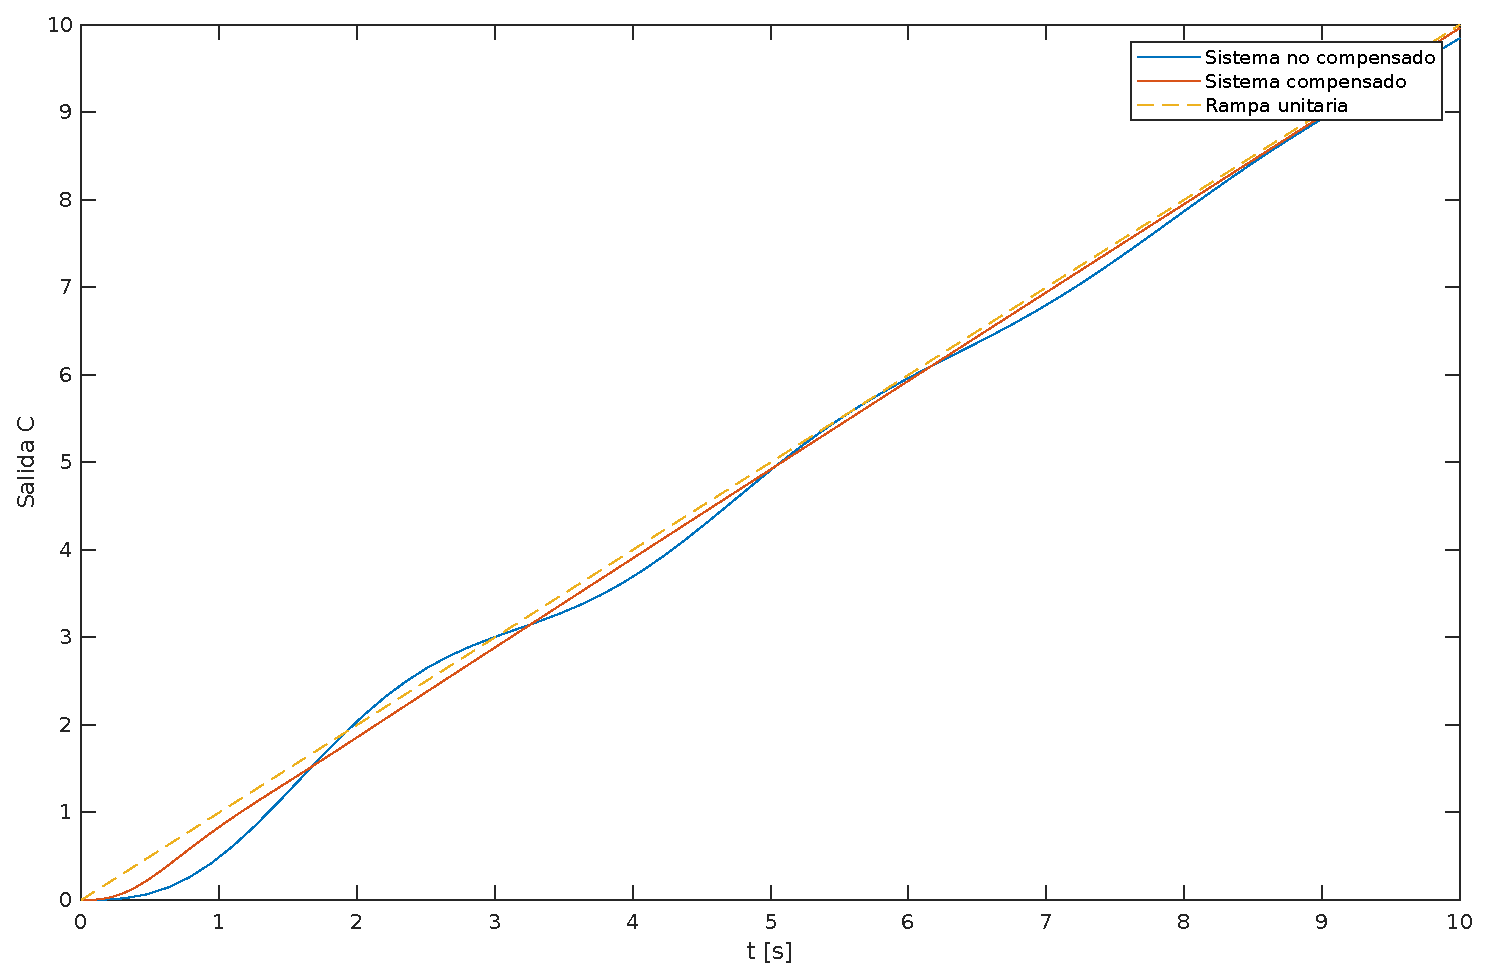
\includegraphics[width=10cm]{images/ejemplo3_comparacion_rampa.eps}
	\end{figure}
	\vspace*{-5mm}
	\centering \footnotesize Respuesta rampa para sistema no compensado y compensado
\end{frame}

\begin{frame}[c]\frametitle{Taller}
	\begin{enumerate}
	 	\item El sistema de control mostrado en la figura representa el control de velocidad de un motor DC, usando un tacómetro de precisión. Se desea mantener una alta precisión en estado estacionario para el control de velocidad. Diseñe un compensador de adelanto para que se satisfagan los siguientes requerimientos: $PO = 10\%$, $T_s \leq 1.5$ s.
	 	\seti
	 \end{enumerate} 
	 \begin{figure}
	 	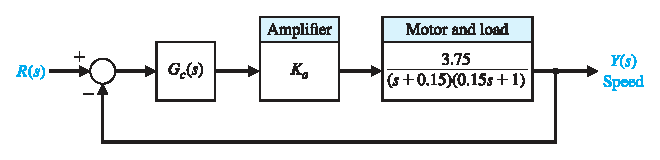
\includegraphics[width=8cm]{images/taller_ejericio1.eps}
	 \end{figure}
\end{frame}

\begin{frame}[c]\frametitle{Taller}
	\begin{enumerate}
		\conti
		\item Un sistema de control con retroalimentación unitaria tiene la siguiente función de transferencia de lazo abierto:
		\begin{equation*}
			G_c(s)G(s) = G_c(s)\frac{5}{s(s^2+5s+12)}
		\end{equation*}
		\begin{itemize}
			\item Diseñe un compensador de atraso usando el LGR tal que la constante de velocidad sea incrementada en 10.
			\item Compare la respuesta paso del sistema no compensado con la del sistema compensado.
		\end{itemize}
		\seti
	\end{enumerate}
\end{frame}

\begin{frame}[c]\frametitle{Taller}
	\begin{enumerate}
		\conti
		\item Un sistema de control con retroalimentación unitaria tiene la siguiente función de transferencia de lazo abierto:
		\begin{equation*}
			G_c(s)G(s) = G_c(s)\frac{160}{s^2}
		\end{equation*}
		\begin{itemize}
			\item Diseñe un compensador de adelanto-atraso usando el LGR tal que los siguientes requerimientos sean satisfechos: $PO \leq 5\%$, $T_s \leq 1$ s, $K_a >= 7500$ (constante de aceleración).
			\item Compare la respuesta paso del sistema no compensado con la del sistema compensado.
		\end{itemize}
		\seti
	\end{enumerate}
\end{frame}

\end{document}